\section{Voraussetzungen}

\subsection{Versuchsziel}

Im Fortgeschrittenen-Praktikum „Quantenkryptographie“ besteht das Versuchsziel
darin, einen digitalen Schlüssel unter Verwendung des BB84-Protokolls
quantenkryptographisch verschlüsselt über eine kurze Distanz zu übertragen.
Die hierfür benötigten quantenmechanischen Zustände werden durch verschiedene
Polarisationen des zur Übertragung verwendeten Laserlichts repräsentiert.

\subsection{Motivation}

Um vertrauliche Informationen auszutauschen, ist die Verschlüsselung das
Mittel der Wahl. Der Sender wird allgemeinhin mit Alice, der Empfänger mit Bob
bezeichnet. Werden während der Überbringung oder Übertragung die Daten von
einem Dritten, der Konvention nach Eve genannt, abgefangen beziehungsweise
mitgelesen, so erhält dieser nicht ohne weiteres Aufschluss über die Informationen.
Die gesicherte Kommunikation ist also nur so lange gewährleistet, wie die zur
Verschlüsselung verwendeten Parameter (der Schlüssel) nur Alice und Bob bekannt
sind. Die Herausforderung verschiebt sich nun von der abhörsicheren
Informationsübermittlung hin zur Frage, wie der Schlüssel ausgetauscht werden
kann.

Bei der asymmetrischen Verschlüsselung wird der Schlüssel in einen privaten und
einen öffentlichen Schlüssel geteilt. Durch die Verwendung von Einmal-Funktionen
entfällt nun die Notwendigkeit einer Schlüsselübergabe. Allerdings kann eine
unbefugte Entschlüsselung nicht prinzipiell ausgeschlossen werden. Man hofft,
dass eine kurzfristige Entschlüsselung auf Grund des hohen Aufwandes nicht möglich
ist. Mit steigender Leistungsfähigkeit der Computer sinkt somit die Sicherheit
der heute verwendeten asymmetrischen Verschlüsselungssysteme, wodurch die Forschung
nach alternativen Lösungsansätzen an Bedeutung gewinnt.

Die symmetrische Verschlüsselung erfordert einen Schlüsselaustausch vor der
Informationsübertragung. Wenn der Schlüssel ebensolang wie die zu verschlüsselnde
Information ist, so ist es prinzipiell unmöglich aus den verschlüsselten Daten
etwas zurückzugewinnen. Man spricht in diesem Fall von dem One-Time-Pad. Gelingt
es allerdings Eve Kenntniss über den Schlüssel zu gewinnen, so ist eine sichere
Verschlüsselung nicht mehr gewährleistet.

Die klassische Kryptographie sieht sich also mit zwei Problemen konfrontiert:
\begin{enumerate}[a)]
 \item Wie kann ein nicht-deterministischer Schlüssel erzeugt werden?
 \item Wie kann ausgeschlossen werden, dass der Schlüssel abgehört wurde?
\end{enumerate}

Die Quantenkryptographie erlaubt die Lösung dieser beiden Probleme. Durch
den der Quantenmechanik eigenen intrinsischen Zufall ist das Vorhersagen
des aus quantenmechanischen Zuständen abgeleiteten Schlüssels nicht möglich.

Außerdem folgt aus dem No-Clone-Theorem, dass der Schlüssel nicht unbemerkt
abgehört werden kann. Hierfür ist es allerdings notwendig, für das Übetragen des
Schlüssels jeweis nur ein Teilchen zu benutzen um einen quantenmechanischen
Zustand zu übertragen.

Nachdem der Schlüssel übertragen wurde und ein Abhören nicht stattgefunden hat,
kann nun auf einem öffentlichen Kanal die chiffrierte Nachricht übermittelt werden.
Für jeden, der nicht im Besitz des Schlüssels ist, ist die verschlüsselte
Botschaft nicht lesbar und daher nutzlos.

\subsection{Physikalische Grundlagen}

Eine mögliche Implementierung des quantenkryptographischen Schlüsselaustausches
wird durch das BB84-Protokoll beschrieben. Hierbei wird die
Polarisationsrichtung von Photonen verwendet, um Quantenzustände zu übertragen.
Prinzipiell können jedoch auch Zeit- und Phasenzustände verwendet werden.

Zunächst erzeugt Alice einzelne Photonen. Diese werden durch
einen Polarisationsfilter geleitet, wodurch die Photonen in einer der beiden
möglichen Basen einen der beiden zueinander orthogonalen Zustände einnimmt.
Die Wahl der Basis erfolgt zufällig.

Die polarisierten Photonen werden nun zu Bob geleitet, der das Licht ebenfalls
mit einem Polarisationsfilter analysiert. Die Wahl der Basis von Bob erfolgt
ebenfalls zufällig. Schließlich können die Photonen, die den Filter passiert
haben, mit einem Detektor nachgewiesen werden.

Stimmen die zufällig gewählten Basen bei Alice und Bob überein, so sind die
Messergebnisse bei Bob zu den gewählten Zuständen bei Alice in der Theorie zu
\SI{100}{\percent} korreliert. Aus diesen Ergebnissen kann schließlich ein
Schlüssel erzeugt werden. Wurden verschiedene Basen verwendet, so müssen die
Messergebnisse bei Bob verworfen werden, da aus ihnen keine Rückschlüsse auf die
gewählten Zustände von Alice gezogen werden können.

Wenn Eve nun versuchen würde, die Polarisation der von Alice gesendeten Photonen
zu messen und ein Photon gleicher Polarisation zu Bob zu senden, müsste Eve
sich zunächst für eine Basis entscheiden müssen. Bei zwei Möglichkeiten wird
Eve in \SI{50}{\percent} der Fälle die falsche Basis verwenden und ein rein
zufälliges Ergebnis messen, welches dann an Bob weitergeleitet werden würde.
Nutzen nun Alice und Bob einen Teil ihres Schlüssels um einen öffentlichen
Vergleich auf Unterschiede des Schlüssels durchzuführen, so kann die Sicherheit
und Richtigkeit des Schlüssels validiert werden. Wenn ein höherer Prozentsatz
des Schlüssels zum Vergleichen genutzt wird, sinkt die Wahrscheinlichkeit, dass
ein Angriff durchgeführt worden ist, jedoch sinkt ebenso die Länge das für die
Verschlüsselung verbleibenden Schlüsselanteils.

Darüber hinaus gibt es noch weitere Möglichkeiten einen Angriff auszuschließen.
So können bestimmte Köder-Lichtpulse (Decoy-States) verwendet werden, um die
Sicherheit weiter zu erhöhen.

\subsection{Versuchsaufbau}

\begin{figure*}[htb]
 \centering
 \includegraphics[page=8,viewport=166 482 445 565,clip,%
  width=0.8\paperwidth,keepaspectratio]{%
  ../doc/crypto3}
 \caption{Aufbau des Experiments}
 \label{fig:aufbau}
\end{figure*}

Der Versuchsaufbau ist schematisch in \fref{aufbau} dargestellt.

Als Einzelphotonenquelle dient ein Laser, dessen Intesität so stark abgeschwächt
wird, dass nur mit einer sehr geringen Wahrscheinlichkeit mehr als ein Photon
gleichzeitig emittiert werden.

Die Photonen werden zunächst durch einen Strahlteiler geleitet, der nur vertikal
porarisierte Photonen passieren lässt und alle anderen Photonen aus der Apparatur
herausleitet. In einem nächsten Schritt passieren die Photonen einen 
elektro-optischen Modulator (EOM), in dem die Photonen durch ein
doppelbrechendes Medium geleitet werden, dessen Brechungsindizes von der
angelegten elektrischen Spannung abhängen. Dieser Spannungswert kann letztlich
softwareseitig variiert werden, wodurch somit das optische Verhalten des
doppelbrechenden Kristalls beeinflusst wird.

Da die Wellenlänge der Photonen konstant \SI{633}{nm} beträgt, kann gezielt
eingestellt werden, ob sich die EOMs wie $λ/4$- oder $λ/2$-Plättchen verhalten.
Nachdem das Licht das erste EOM passiert hat, verbleiben je nach gewähltem
Spannungswert bei Wahl von Basis 1 horizontal oder vertikal und bei Wahl von
Basis 2 rechts- bzw. links-zirkular polarisierte Photonen.

Ein Nachweis, dass die gewählten Polarisationen innerhalb des BB84-Protokolls
verwendet werden können, ist im Anhang \ref{sec:zirkular} zu finden.

Auf der Seite von Bob wird das eintreffende Licht zunächst durch einen weiteren
EOM geleitet. Hier wird die Polarisationsrichtung des Lichts erneut um einen
gewissen Winkel gedreht, der mit einer Spannung softwareseitig geregelt werden
kann. Anschließend wird der Lichtstrahl erneut durch einen Strahlteiler
geleitet, nachdem nur die vertikal polarisierten Anteile verbleiben.
Schließlich werden die Photonen mit einer Avalanche-Photodiode (APD)
registriert.
